\documentclass[conference]{IEEEtran}
\IEEEoverridecommandlockouts
%The preceding line is only needed to identify funding in the first footnote. If that is unneeded, please comment it out.


%\usepackage{cite}
\usepackage{amsmath,amssymb,amsfonts}
\usepackage{algorithmic}
\usepackage{graphicx}
\usepackage{textcomp}
\usepackage{xcolor}

% JH/zusätzliche Packages, die ich verwendet habe
\usepackage{hyperref}


% JH/Definition eigener Befehle
\newcommand{\R}{\mathbb{R}}
\newcommand{\N}{\mathbb{N}}
\newcommand{\TSShoch}{\mathhbb\textsuperscript{}}
%\textsuperscript{2}

\def\BibTeX{{\rm B\kern-.05em{\sc i\kern-.025em b}\kern-.08em
    T\kern-.1667em\lower.7ex\hbox{E}\kern-.125emX}}
    
    
\usepackage[backend=bibtex, style=numeric]  
           {biblatex}
\addbibresource{Literature.bib}   
    
\begin{document}

\title{Diode pumped $Pr^{3+}$:LiYF4 lasers emitting at 640 nm, 604 nm and 523 nm\\
}

\author{Niklas H.}

\maketitle

\begin{abstract}
In this report, a Praseodymium doped LiYF4 (Pr:YLF) laser consisting of a hemispheric cavity of 50 mm (640 nm) or 100 mm (604nm/523nm) and a 6mm long longitudinally pumped crystal (0.8 at\% doping) is reported. Depending on the mirror set used, the 640 nm ($^3P_0$ to $^3F_2$), 607 nm ($^3P_0$ to $^3H_6$) and 523 nm ($^3P_0$ to $^3H_5$) lines of the $Pr^{3+}$-Ion can be amplified. For the red line, an OC with 1.8\%T resulted in X.
\end{abstract}

\begin{IEEEkeywords}
LiYF4 Laser, DPSS Laser, Pr:YLF Laser
\end{IEEEkeywords}
%-------------------------------------------------------------------------------------
\section{Introduction}
%-------------------------------------------------------------------------------------

Since the introduction of lasers in 1960 by Theodore Maiman, many gain media for obtaining optical gain and therefore laser action have been introduced. One these media is LiYF4 doped with $Pr^{3+}$-Ions (Pr:YLF), which is able to operate at multiple lines, e.g. 720nm, 607nm, 640nm and 523nm, which is why special research efforts have been directed towards this material. It is also one of the few gain media which directly (without frequency doubling) emit visible light and also are pumped by visible light. Furthermore, continous wave UV emission by intracavity doubling has been reported \cite{Richter.2006}\cite{Gun.2011}. For this report, the 640 nm ($^3P_0$ to $^3F_2$), 607 nm ($^3P_0$ to $^3H_6$) and 523 nm ($^3P_0$ to $^3H_5$) transitions are of relevance. The $Pr^{3+}$-Ion reaches the excited state $^3P_0$ by being excited to the $^3P_2$ state and fastly relaxing to $^3P_0$. The excitation process is performed most efficiently by using 444nm pumplight. Since InGaN laser diodes emit around this exact wavelength and are commercially available at several watts of optical power, they have been used extensively for pumping Pr:YLF lasers \cite{Xu.2013}\cite{Krankel.2016}\cite{Bellancourt.2010}\cite{Luo.2018}\cite{Muller.2011}. For linear end-pumped resonator designs using InGaN laser diodes, slope efficiencies of 49\% for 523 nm, 40\% at 607 nm and 57\% for 640 nm have been reported \cite{Luo.2016}. 
\section{Experimental setup}
The resonator setups for amplifying the 607 nm and 640 nm lines were a standard hemispherical cavity with the a concave outcoupling mirror as reported in e.g. \cite{Luo.2016} and \cite{Bellancourt.2010}. The setup is depicted in figure \ref{setup607640}.
\begin{figure}[h]
	\centering
	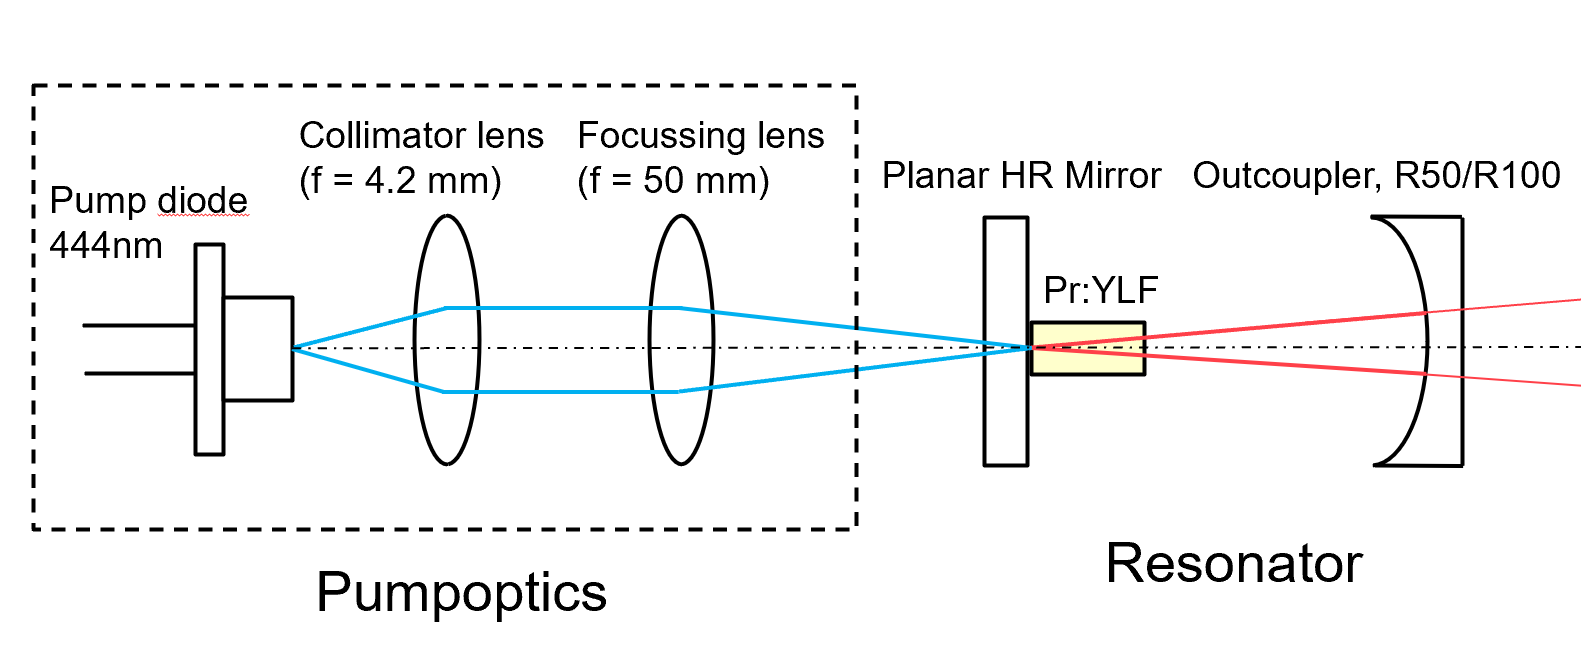
\includegraphics[width=0.4\textwidth]{img/setup607640}
	\caption{Setup for 607 nm and 640 nm laser output}
	\label{setup607640}
\end{figure}
For 607 nm and 640 nm output couplers (OC) with 1\% T and 1.8\% T were used. The radius of curvature (ROC) and therefore cavity length was 100 mm and 50 mm respectively. The Pr:YLF crystal used had a doping concentration of 0.8 at\% and was 6 mm long. The faces of the crystal were coated with an antireflection coating for 444 nm and 500 nm - 720 nm. It was placed directly in front of the high reflecting mirror (HR), with about 2 mm of air between them. The crystal was glued into an aluminium holder using a thermal glue, in order to passively cool it down. This holder was designed to be water-cooled as well, but this did not prove to be necessary at the power levels produced by the pump diode. A HR with high transmission at 444 nm and high reflectivity at 600 nm - 700 nm was used. The crystal was pumped longidutinally.\\
For pumping, a Nichia NDB7875 laser diode was used. The diode was selected to have an output wavelength of 444 nm at 1.5 A, which corresponds to ~2 W of output power. The pump diode was collimated using an aspheric lens with f = 4.2 mm (Thorlabs A390TM-A) and focussed into the crystal via a bi-convex lens with f = 50 mm (Thorlabs LB1844-A). Both pump optics were delivered with a VIS antireflection coating. The pump diode was water cooled. Since the absorption coefficient of Pr:YLF is highly dependent on polarization \cite{Xu.2013}, the pump diode was rotated until the absorption peaked and then locked rotationally to match the pump polarization and the crystal orientation. \\
Due to availability issues, a different setup for obtaining 523 nm laser output was implemented. This setup is depicted in figure \ref{setup523}.
\begin{figure}[h]
	\centering
	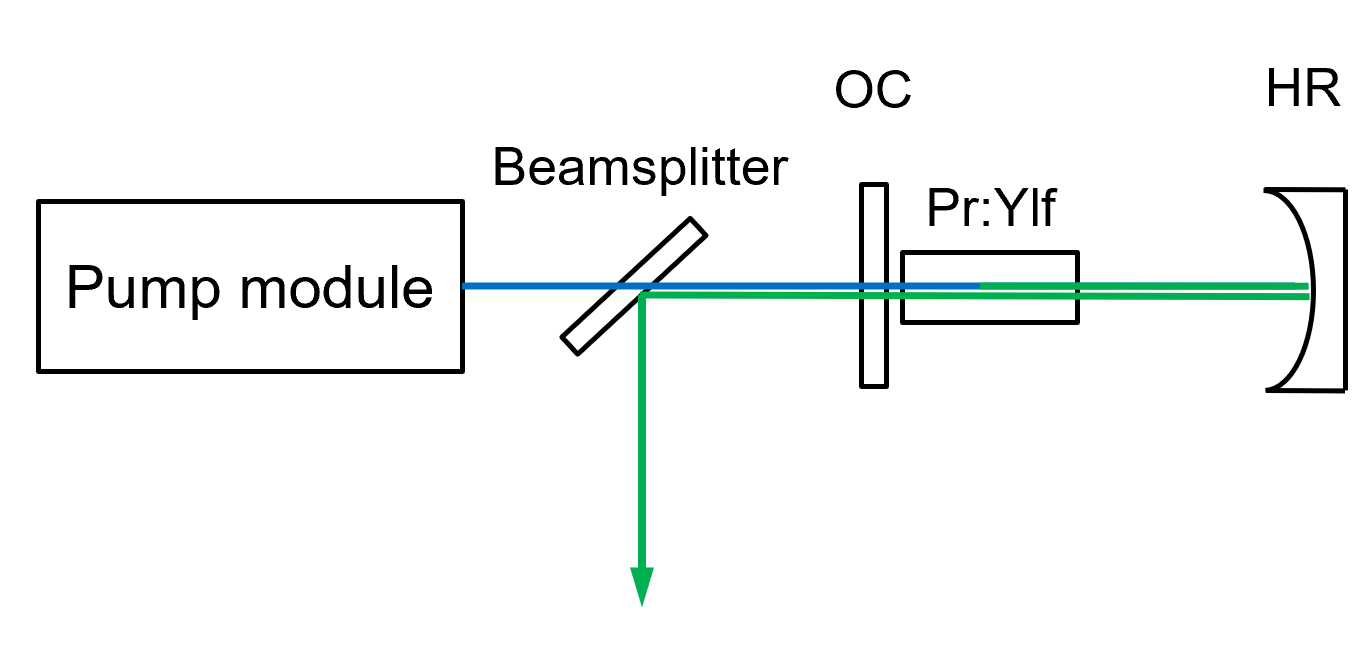
\includegraphics[width=0.4\textwidth]{img/setup523}
	\caption{Setup for 523 nm laser output}
	\label{setup523}
\end{figure}
In this case, the concave mirror was coated with a very high reflective coating ($\geq$ 99.9\% R) for 523 nm. The plane mirror was used as the output coupler, with a reflectivity of about 0.5\% for 523 nm. A beamsplitter with high transmission for the pumplight and high reflectivity for 523 nm was installed to guide the laser beam out of the setup. 
\section{Results}
\section{Conclusion}
%-------------------------------------------------------------------------------------
%-------------------------------------------------------------------------------------
%\section*{References}
\printbibliography
%-------------------------------------------------------------------------------------
%-------------------------------------------------------------------------------------
\end{document}
